\documentclass[a4paper,12pt]{article} 
\usepackage[utf8]{inputenc}
\usepackage[margin=1.2in]{geometry}
\usepackage{amsmath, amssymb}
\usepackage{graphicx}
\usepackage{setspace}
\renewcommand{\baselinestretch}{1.5} 
\graphicspath{ {../pdf/} {/Users/davidubaldo/Desktop/latex/} }
\usepackage[portuguese]{babel}
\usepackage{indentfirst}
\usepackage{wrapfig}
\usepackage{apacite}

\begin{document}

\begin{titlepage}
    \begin{center}
    		{\setstretch{1.0}
        \vspace*{0.5 cm}
            
        \Huge
        \textbf{Projeto LaTeX}
            
        \vspace{0.5cm}
        \LARGE
        Uma breve olhada na disciplina de \textbf{Automação Inteligente}
            
        \vspace{1.5cm}
            
        \textbf{David Londes}
            
        \vfill
            
        Trabalho apresentado para a disciplina de\\
        Introdução à Computação
            
        \vspace{0.8cm}
            
        
\includegraphics[scale=0.3]{cinufpe}
            
        \Large
        Centro de Informática\\
        Universidade Federal de Pernambuco\\
        Brasil\\
        19 de outubro de 2020
            }
    \end{center}
\end{titlepage}



	\begin{center}
		\LARGE
		\textbf{Introdução}
	\end{center}
	\vspace*{0.5 cm}
	\par 
		O sistema LaTeX é uma linguagem de marcação que lida com a composição e a renderização de textos. Também pode ser arbitrariamente estendida por meio de pacotes, a fim de desenvolver macros personalizadas, como novos ambientes e comandos.
	\par
		Este trabalho visa explorar essa poderosa linguagem por meio de uma apresentação da disciplina \textbf{Automação Inteligente}. Aqui será mostrado sua relevância na atualidade e sua relação com as outras disciplinas ofertadas pelo CIn.
		
	\clearpage
	
	\begin{center}
		\LARGE
		\textbf{Desenvolvimento}
	\end{center}
	\vspace*{0.5 cm}
	
	\section{O que é Automação Inteligente?}

		Automação Inteligente é uma combinação das tecnologias de automação de processos robóticos (RPA) e de inteligência artificial (IA) que, juntas, capacitam a automação de processos ponta a ponta e aceleram a transformação digital.	
		
De modo que seja possível estender a automação de processos de grandes magnitudes, a automação inteligente combina a execução de tarefas de RPA com aprendizado de máquina e recursos de análise de descoberta automática de processos. Também engloba tecnologias cognitivas, como: visão computacional, processamento de linguagem natural, e lógica fuzzy.

	\begin{figure}[h!]
	\centering
  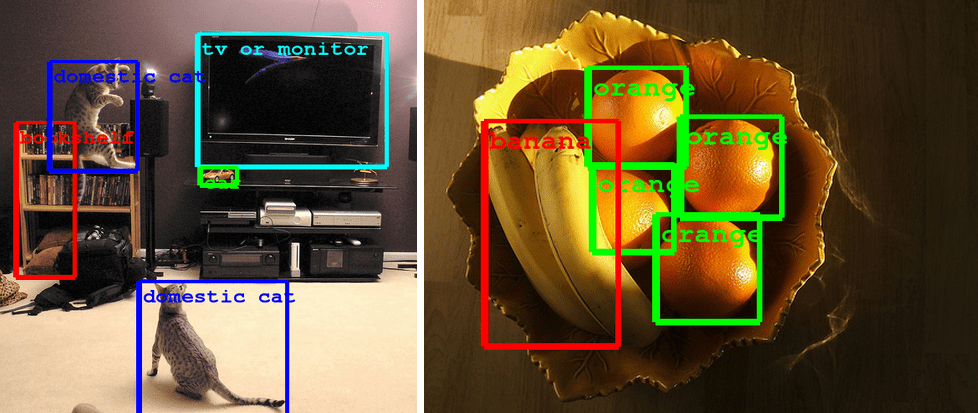
\includegraphics[width=0.8\textwidth]{computer-vision}
   \scriptsize{ \caption{ Exemplo de visão computacional. Fonte: https://www.unite.ai/what-is-computer-vision}}
\end{figure}


A automação inteligente abrange toda o campo da automação, tornando qualquer processo de negócios de front ou back-office mais efetivo, também orquestra o trabalho entre equipes humanas combinadas de bots.

	\section{Os quatro pilares da automação inteligente}
	
 

\begin{description}
  \item[1º Pilar: Gestão de Processos de Empresariais] \hfill \\ O objetivo do GPE é garantir que a infraestrutura operacional e dos processos nos negócios funcione corretamente. Portanto, atua como uma camada de base na organização, automatizando o comportamento de processos complexos que exigem que as pessoas intervenham na entrada de dados e na tomada de decisões. Exemplos são: a utilização de sistemas em momentos específicos como cálculos ou integrações, controle de ações e geração de dados e armazenamento.
  
  
  \item[2º Pilar: Automação de Processos Robóticos ] \hfill \\ A RPA é uma tecnologia que visa reduzir a intervenção humana em aplicações computacionais, principalmente em tarefas repetitivas que variam muito pouco a cada interação. Essa tecnologia é adequada para substituir tarefas manuais simples e repetitivas, como entrada de dados em aplicativos. Isso significa que os funcionários têm mais tempo para se concentrar em outros ramos de valor para a empresa, como a tomada de decisões ou a melhoria das relações com os clientes.
  
  
  \item[3º Pilar: Inteligência Artificial ] \hfill \\ A Inteligência Artificial é a simulação da inteligência humana por máquinas.
Em outras palavras, é a disciplina que tenta criar sistemas capazes de aprender e raciocinar como um ser humano. A IAl engloba outros conceitos como Aprendizado de Máquina, Aprendizado Profundo, Processamento de Linguagem Natural (PNL), Reconhecimento Visual, Big Data, etc.

\item[4º Pilar: Integrações] \hfill \\ A conexão e integração entre sistemas é parte essencial da Automação Inteligente. Por meio de uma interface, é possível integrar todos os elementos da automação, de modo que tudo fique mais fácil de ser administrado.

\end{description}

	\begin{figure}[h!]
	\centering
  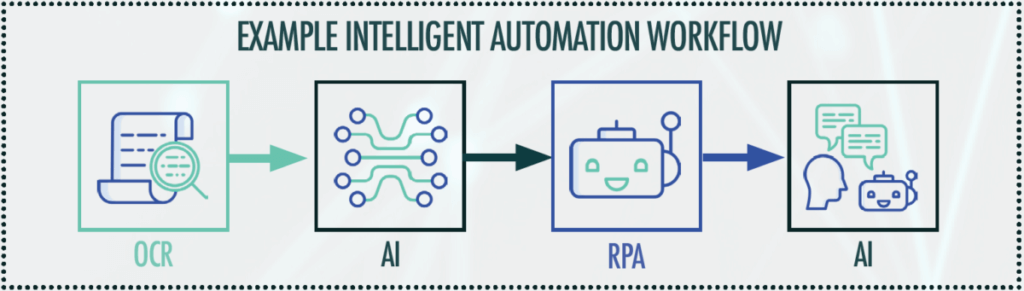
\includegraphics[scale=0.27]{automationworkflow}
  
   \tiny{ \caption{ O proceso da automação inteligente. Fonte: https://burniegroup.com/intelligent-automation-key-benefits-for-your-business/ }}
	\end{figure}
	
	\begin{section}{Relação com as outras disciplinas ofertadas pelo CIn}
	A automação inteligente tem uma relação muito forte com tudo que envolve inteligência artificial e negócios. Apesar dessa disciplina não ter nenhum pré ou co-requisito no CIn, ela está fortemente ligada com outras disciplinas de IA, como: IF669 – Aprendizagem de Máquina; IF752 – Visão Computacional; IF703 – Agentes Autônomos;  IF684 – Sistemas Inteligentes; IF704 – Processamento de Linguagem Natural.
	\end{section}

		\clearpage
		
	\bibliographystyle{apacite}
	\bibliography{referencias}	
		
\end{document}
